\documentclass{report}
\usepackage[T1]{fontenc}
\usepackage{color}
\usepackage{amssymb}
\usepackage{pdfpages}
\usepackage{amsmath}
\usepackage{eurosym}
\usepackage{graphicx}
\usepackage{textcomp}
\usepackage{listings}
\usepackage{epigraph}
\usepackage{setspace}
\usepackage{array}
\usepackage{gensymb}
\usepackage{tikz}
\usepackage[some]{background}
\usepackage{geometry}
\usepackage[english]{babel}


\begin{document}
\renewcommand{\chaptername}{Part}
\renewcommand{\thechapter}{\Roman{chapter}}

%\usepackage{lmodern}
%\usepackage{xspace}
%\usepackage{hyperref}

\definecolor{sup_strip_color}{rgb}{0.80,0.80,0.80}
\definecolor{inf_strip_color}{rgb}{0.00,0.00,0.00}

\DeclareFixedFont{\bigsf}{T1}{phv}{b}{n}{0.8cm}

\makeatletter                       
\def\printauthor{%                  
    {{\large \@author}}}              
\makeatother

\author{Zohour \textsc{Abouakil} ~\\ Sofia \textsc{Boutahar} ~\\ David \textsc{Courtinot} ~\\ Xiaowen \textsc{Ji} ~\\ Fabien \textsc{Sauce}}

\begin{titlepage}

\newgeometry{left=1cm,right=4cm,bottom=0cm}
\begin{tikzpicture}[overlay,remember picture]
% the black stripe with the title
\node[
  fill=inf_strip_color,
  anchor=north west,
  text width=\paperwidth,
  text height=2cm,
  text depth=2cm,
  inner xsep=1cm,
  font=\color{white}\bigsf 
  ] 
 at ([yshift=-2.5cm]current page.north west) (blackrect) {Design review - Iteration 1 - Version 2};
% the khaki stripe
\path[fill=sup_strip_color] 
  (blackrect.north west) rectangle ++(\paperwidth,2.5cm);
\end{tikzpicture}

\vspace*{4.5cm}

\noindent
\begin{minipage}{0.35\linewidth}
    \begin{flushright}
        \printauthor
    \end{flushright}
\end{minipage} \hspace{15pt}
%
\begin{minipage}{0.02\linewidth}
    \rule{1pt}{175pt}
\end{minipage} \hspace{-10pt}
%
\begin{minipage}{0.6\linewidth}
\vspace{5pt}
\newenvironment{test}{\begin{center}}{\end{center}}
\hspace{10pt}
\begin{minipage}{\linewidth} 
\textbf{Reference :} model-checking.design ~\\
January $30^{th}$ 2015
\end{minipage}
\end{minipage}

\vspace{8cm}
\begin{minipage}{0.20\linewidth}
    \begin{flushright}
       
        \begin{tabular}{ll}
	 \textit{Signatures} & \\
            & \textbf{Quality responsible :} \\
            & \textbf{Clients :} \\
        \end{tabular}
    \end{flushright}
\end{minipage}

\end{titlepage}
\restoregeometry
\tableofcontents
\newgeometry{left=2.1cm,right=2.1cm}
\chapter{AST and CFG representations}

\paragraph{}
\hspace{4mm}\textnormal{}

\section{Transitional reprensentation of the Clang AST}

\subsection{Parse the Clang AST file}

\paragraph{}
\hspace{4mm}\textnormal{At first, we have considered using XML parsing libraries to parse the XML version of the Clang AST. However, 
this type of output is no longer supported by the newest versions of the Clang compiler and all the existing tools
provide partial support at best. Hence, we decided using the regular AST file and parse it line by line 
with a custom parser.}

\paragraph{}
\hspace{4mm}\textnormal{We have identified three main kinds of nodes in the AST. Each one is associated to a specific class which extends ASTNode :}

\vspace{4mm}
\begin{itemize}
\item nodes consisting in an type name, an id, a code pointer pointing the relevant lines of the code and some
metadata that depend on the type of the node. These are represented by the ConcreteASTNode class\vspace{1mm}
\item <<<NULL>>> children, represented by the NullASTNode class\vspace{1mm}
\item other kind of nodes, prior to class declaration for example. These are represented by OtherASTNode\vspace{1mm}
\end{itemize}

\begin{center}
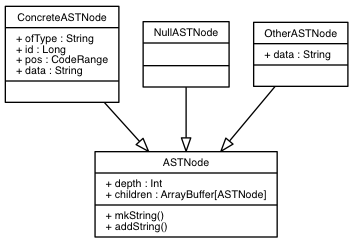
\includegraphics[scale=0.8]{ASTNode.png}
~\\~\\Figure I.1 - Inheritance relationships between the classes used to represent the AST
\end{center}

\paragraph{}
\hspace{4mm}\textnormal{The file will be parsed and converted in a tree data-structure which nodes are of type ASTNode.}

\subsection{From ASTNode to ProgramNode}

\subsubsection{\textbf{Decl} class hierarchy}

\subsubsection{Partie \textbf{Stmt}}

\paragraph{}
\hspace{4mm}\textnormal{}

\begin{center}
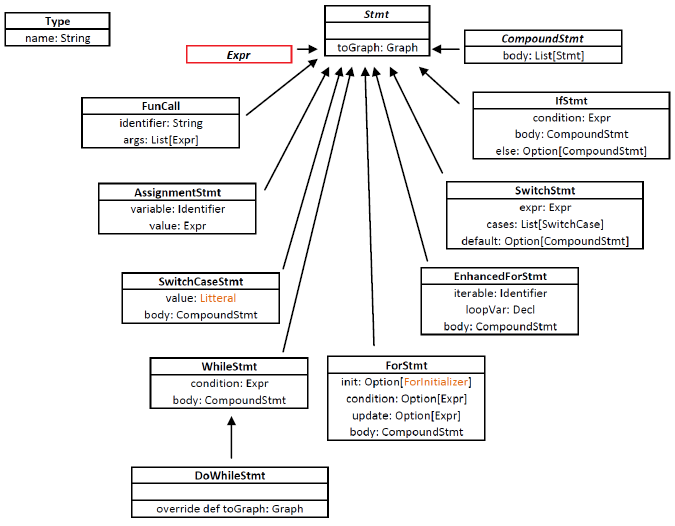
\includegraphics[scale=0.9]{data/stmt.png}
~\\~\\Figure I.2 - 
\end{center}

\paragraph{}
\hspace{4mm}\textnormal{}

\begin{center}
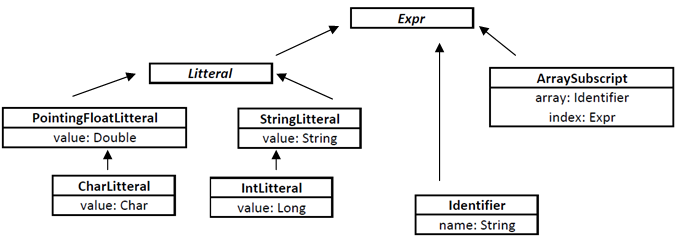
\includegraphics[scale=0.9]{data/expr1.png}
~\\~\\Figure I.3 - Diagramme de classe partiel de la partie \textbf{Expr}
\end{center}

\paragraph{}
\hspace{4mm}\textnormal{}

\begin{center}
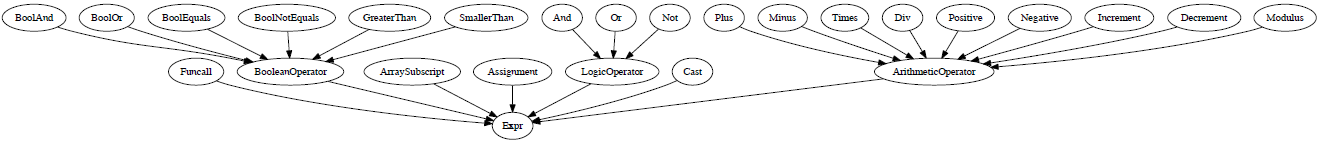
\includegraphics[scale=0.5]{data/expr2.png}
~\\~\\Figure I.4 - Diagramme de classe plus fourni (mais toujours incomplet) de la partie \textbf{Expr}
\end{center}

\subsubsection{Remarques importantes :}

\vspace{4mm}
\begin{itemize}
\item \vspace{1mm}
\end{itemize}

\begin{center}
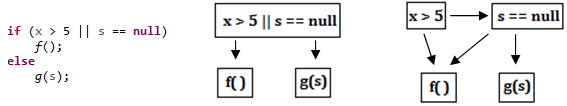
\includegraphics[scale=0.85]{data/fail-fast.png}
~\\~\\Figure I.5 - 
\end{center}

\paragraph{}
\hspace{4mm}\textnormal{}

\section{AST to CFG}

\chapter{Model checking}

\end{document}
